\documentclass{article}
\setlength\parindent{0pt}
\usepackage{graphicx} % Required for inserting images
\usepackage[a4paper, total={7in, 7in},margin=1in]{geometry}
\usepackage{subcaption}
\usepackage{float}
\usepackage{hyperref} 
\usepackage{xurl}


\title{\textbf {A Comparative Study of Non-parallelized and  Parallelized Random Forest Model}}
\author{Sri Lakshmi Bathina, Abhishek Siriki, Nikita Rego }
\date{December 10, 2023}

\begin{document}
\maketitle
\section{Background on Random Forest model}
Random Forest is a sophisticated machine learning technique that enhances predictive modeling capabilities. By pooling the collective wisdom of multiple decision trees built on random subsets of the data-set during the training stage, this algorithm boosts overall accuracy and robustness. This ensembling approach helps mitigate over-fitting issues and enables better adaptation to unseen, complex data. Specifically, Random Forest shines when dealing with high-dimensional data-sets, large volumes of information, and providing meaningful insight into the importance of individual features. Its exceptional performance and flexibility have made it a valuable asset across various disciplines, allowing for more reliable and accurate predictions in difficult scenarios.

\section{Need for parallelization in random forest model}
Essentially, there are 4 main phases when building a machine learning model (excluding data pre-processing and model deployment). These phases are 
\begin{enumerate}
    \item Training Phase
    \item Model Tuning Phase
    \item Validation Phase
    \item Testing phase. 
\end{enumerate}
These 4 phases take varied amounts of time depending on the data and the model being built. Parallelization of these 4 phases should allow for shorter time frame to generate models \\ 

Parallelization is crucial in Random Forest models to make them work faster and use computer resources better. It involves spreading out the creation of decision trees across many cores simultaneously. This is really helpful when dealing with big sets of data, making the model quicker and avoiding delays. Using parallelization not only speeds up the process but also lets us explore different settings for the model more efficiently. In short, parallelization is a vital technique in Random Forests, making them work faster and smarter with the technology we have today.

\section{Methods of Parallelization employed}
In Python, \textbf{multiprocessing.Pool} is an all-purpose tool for distributing tasks across multiple processes, making it easier to perform parallel computations. Meanwhile, the \textbf{n\textunderscore{}jobs} parameter is frequently employed in libraries like scikit-learn to manage the number of simultaneous tasks, particularly when training machine learning models. \\ 
Although multiprocessing.Pool offers more flexibility and can be utilized in various parallelization situations, n\textunderscore{}jobs provides a user-friendly alternative with a streamlined interface specifically designed for executing certain tasks in parallel. The choice between these two methods hinges on the particular requirements of the code being parallelized and the nature of the task at hand. Together, both approaches facilitate effective parallelization techniques in Python.

\section{Building a model}
We chose to build the model on the data-set titled \textbf{``fmendes-DAT263x-demos''} from Kaggle. This data-set contains data related to Correlations between calories burnt, exercise and body type. \\
To start with we imported the necessary module and packages with which we would build our model. We then conducted our data pre-processing and visualization to understand the data. We then commenced to build a broken down version of the serial code to ensure that we were building the model correctly. We later wrote the code to parallelize the 3 phases of the model.\\

The code for this can be found in the file \textbf{``Calories\textunderscore{}Burnt\textunderscore{}Prediction.ipynb"}

\section{Results}

\subsection{Initial Model plots}

We first did 2 individual plots to mark the time taken for training, prediction, cross-validation and the accuracy of the models with and without parallelization in pool and n\textunderscore{}jobs. \\

*Note : For accuracy we calculated the mean absolute error (MAE); the lower the value of MAE, the more accurate the predictions of the model are \\

\begin{figure}[H]
\begin{subfigure}{0.6\textwidth}
\hspace{-0.75cm}
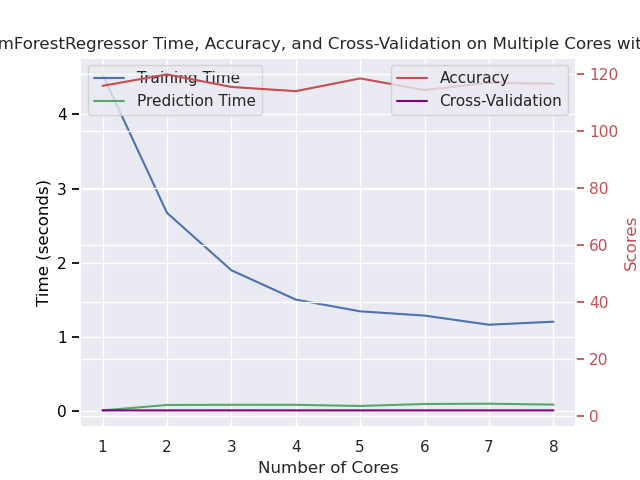
\includegraphics[width=0.8\linewidth, height=6cm]{n_jobs-plot.png} 
\caption{n\textunderscore{}jobs Plot}
\label{fig:subim1}
\end{subfigure}%
\begin{subfigure}{0.6\textwidth}
\hspace{-0.75cm}
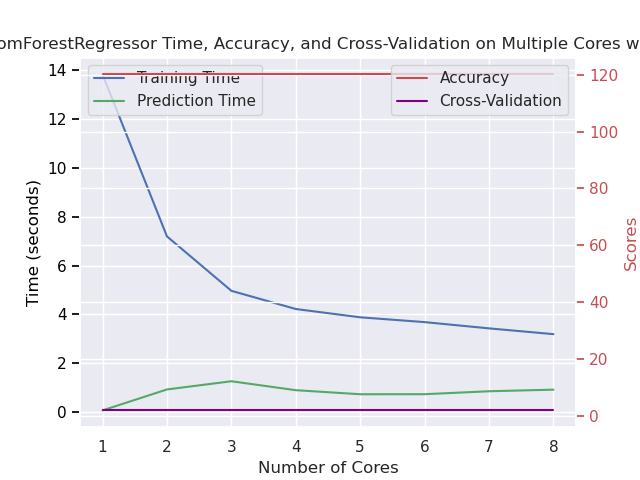
\includegraphics[width=0.8\linewidth, height=6cm]{Pool-plot.png}
\caption{Pool Plot}
\label{fig:subim2}
\end{subfigure}

\caption{Random Forest Regressor Time, Accuracy, and Cross-Validation on Multiple Cores}
\label{fig:image1}
\end{figure}



In \textbf{`plot (a)'} of Figure 1, we can see that as the number of cores increase, the time take for training of he model decreases. At about 6 cores, the time takes becomes closely flat-lined. the time for prediction and cross-validation is constant across the number of cores. The accuracy, however, continues to vary. \\

In \textbf{`plot(b)'} of figure 1, we once again see that as the number of cores increase, the time take for training of he model decreases. However, unlike the case with n\textunderscore{}jobs, the time taken does not flat-line. The time taken for cross-validation and the Accuracy of the model is more or less even along the cores; neither increasing nor decreasing.The time take for prediction, on the other had increases a bit when up to 3 cores are used and then is almost the same along the other cores.\\

One thing of note was that once parallelized with n\textunderscore{}jobs, the time taken tarted from 4 seconds and dropped till 2 seconds while in the case of the parallelization with pool, the time initially started from 14 seconds and dropped to about 3 seconds. Another thing to note was that after a certain point, of training, random forest tends to over-fit the data so plotting the accuracy was not as helpful as if should be.

\subsection{Plots with Hyper-parameter Tuning}
Hyper-parameter tuning in Random Forest involves systematically searching for the optimal values of parameters like the number of trees, depth of trees, and minimum samples per leaf to enhance the model's performance. Hyper-parameter optimization through GridSearchCV in Random Forest can be an extensive endeavor due to the need to explore numerous combinations of hyper-parameters, thereby increasing computational resources required.So with the aim to reduce the time to build a random forest model with tuning the hyper parameters, we parallelized it with both pool and n\textunderscore{}jobs and plotted the results in 3 figures

\subsubsection{Training plot with hyper-parameter tuning}
\begin{figure}[h]
    \centering
    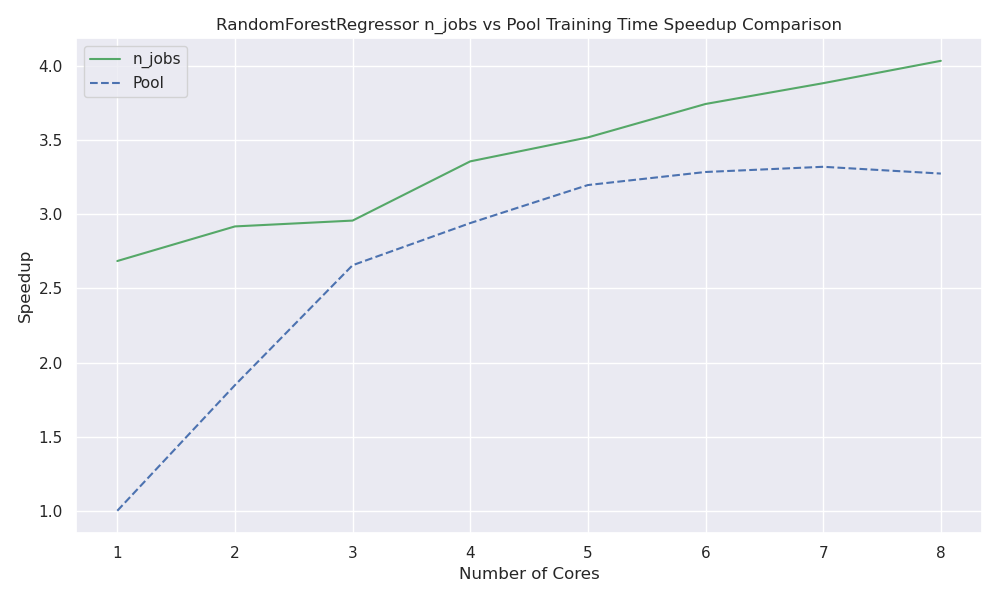
\includegraphics[width=0.90\linewidth]{training_time_n_jobs_vs_pool_speedup_comparison.png}
    \caption{n\textunderscore{}job Vs pool speedup in model training}
    \label{fig:imagea}
\end{figure}
In \textbf{Figure 2}, we can see that in both types of parallelization, as the number of cores increase, the speedup for training also increases. In `n\textunderscore{}jobs', the speedup appears to be a bit more linear as compared to the speed up with `pool' parallelization. While the speedup due do parallelization with `n\textunderscore{}jobs' increases gradually, the speedup with `pool' is initially steep and then lessens as the number of cores increase.

\subsubsection{Validation plot}
\begin{figure}[H]
    \centering
    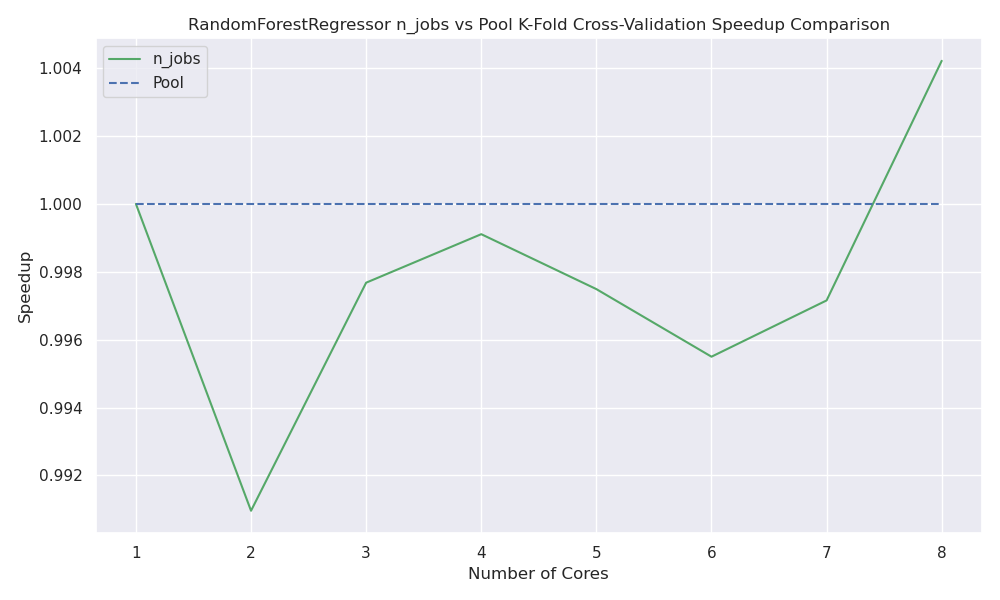
\includegraphics[width=0.90\linewidth]{k-fold_cross-validation_n_jobs_vs_pool_speedup_comparison.png}
    \caption{n\textunderscore{}job Vs pool speedup in model validation}
    \label{fig:enter-label}
\end{figure}
In \textbf{Figure 3}, we can see that there is virtually no speed up in model validation parallelized with `pool'. In `n\textunderscore{}jobs', the speedup is extremely erratic. 

\subsubsection{Testing plot}
\begin{figure}[H]
    \centering
    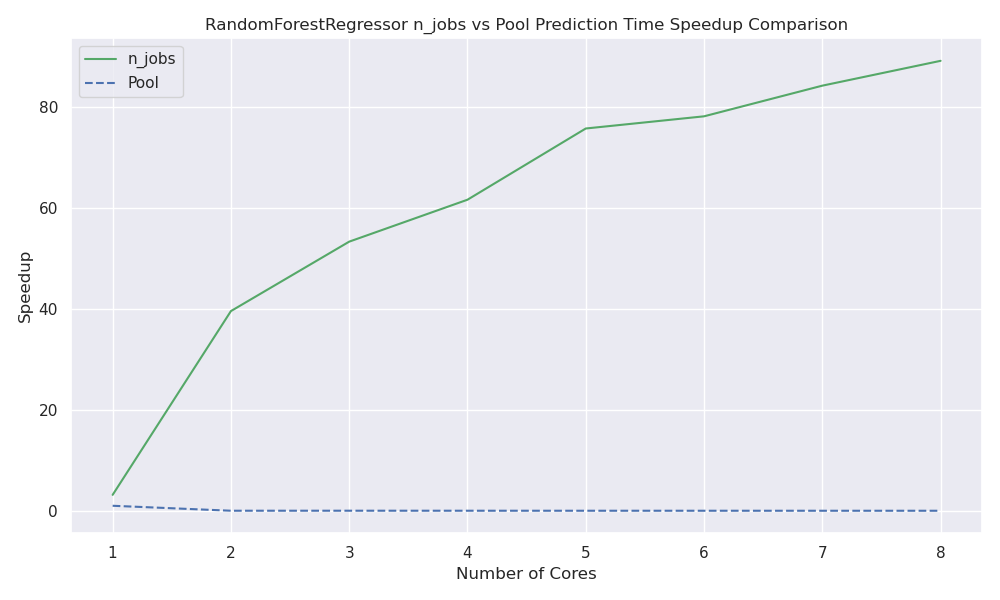
\includegraphics[width=0.90\linewidth]{prediction_time_n_jobs_vs_pool_speedup_comparison.png}
    \caption{n\textunderscore{}job Vs pool speedup in model testing}
    \label{fig:enter-label}
\end{figure}

In \textbf{Figure 4}, we once again see virtually no speed up in model validation parallelized with `pool'.In fact, the speed up appears to decrease a bit as we go from 1 core to 2 cores. On the other hand, in `n\textunderscore{}jobs', the speedup  is seemingly gradual. 

\subsection{Reasoning behind the results}
Although the speedup results in both cases varied, we expect this due to the limited amount of data we have used. Since we have only 15000 records, it was eminent that we would not see that much of a speed up due to the following reasons:

\begin{enumerate}
\item When parallelizing tasks, additional overhead costs, including data partitioning, inter-process communication, and result consolidation, can significantly impact overall execution time. These expenses might outweigh the advantages of parallel processing for smaller data-sets.
\item As an ensemble learning approach, random forest's parallelization potential may not be fully realized due to the inherent complexity involved in creating separate decision trees. Smaller data-sets may not provide adequate data to divide efficiently among multiple processors.
\item Parallelization efficacy typically increases with larger data-sets, providing more balanced workloads that enable efficient division of labor among multiple tasks.
\end{enumerate}
\subsection{References}


\begin{itemize}
\item \texttt{\nolinkurl{https://www.kaggle.com/datasets/fmendes/fmendesdat263xdemos}}
\item \texttt{\nolinkurl{https://docs.python.org/3/library/concurrent.futures.html}}
\item \texttt{\nolinkurl{https://stackabuse.com/random-forest-algorithm-with-python-and-scikit-learn/}}
\item \texttt{\nolinkurl{https://scikit-learn.org/stable/modules/generated/sklearn.ensemble.RandomForestClassifier.html}}
\item \texttt{\nolinkurl{https://hutsons-hacks.info/parallelisation-of-sci-kit-learning-python-models}}
\item \texttt{\nolinkurl{https://scikit-learn.org/stable/modules/ensemble.html##random-forests}}
\item \texttt{\nolinkurl{https://towardsdatascience.com/hyperparameter-tuning-the-random-forest-in-python-using-scikit-learn-28d2aa77dd74}}
\item \texttt{\nolinkurl{https://docs.python.org/3/library/multiprocessing.html}}
\item \texttt{\nolinkurl{https://joblib.readthedocs.io/en/latest/generated/joblib.Parallel.html}}
\end{itemize}

\end{document}
